\documentclass[]{article}
\usepackage{lmodern}
\usepackage{amssymb,amsmath}
\usepackage{ifxetex,ifluatex}
\usepackage{fixltx2e} % provides \textsubscript
\ifnum 0\ifxetex 1\fi\ifluatex 1\fi=0 % if pdftex
  \usepackage[T1]{fontenc}
  \usepackage[utf8]{inputenc}
\else % if luatex or xelatex
  \ifxetex
    \usepackage{mathspec}
  \else
    \usepackage{fontspec}
  \fi
  \defaultfontfeatures{Ligatures=TeX,Scale=MatchLowercase}
\fi
% use upquote if available, for straight quotes in verbatim environments
\IfFileExists{upquote.sty}{\usepackage{upquote}}{}
% use microtype if available
\IfFileExists{microtype.sty}{%
\usepackage{microtype}
\UseMicrotypeSet[protrusion]{basicmath} % disable protrusion for tt fonts
}{}
\usepackage[margin=1in]{geometry}
\usepackage{hyperref}
\hypersetup{unicode=true,
            pdftitle={MVA Final Project},
            pdfauthor={Javier Ferrando Monsonis; Marcel Porta Valles; Mehmet Fatih ??agil},
            pdfborder={0 0 0},
            breaklinks=true}
\urlstyle{same}  % don't use monospace font for urls
\usepackage{color}
\usepackage{fancyvrb}
\newcommand{\VerbBar}{|}
\newcommand{\VERB}{\Verb[commandchars=\\\{\}]}
\DefineVerbatimEnvironment{Highlighting}{Verbatim}{commandchars=\\\{\}}
% Add ',fontsize=\small' for more characters per line
\usepackage{framed}
\definecolor{shadecolor}{RGB}{248,248,248}
\newenvironment{Shaded}{\begin{snugshade}}{\end{snugshade}}
\newcommand{\KeywordTok}[1]{\textcolor[rgb]{0.13,0.29,0.53}{\textbf{#1}}}
\newcommand{\DataTypeTok}[1]{\textcolor[rgb]{0.13,0.29,0.53}{#1}}
\newcommand{\DecValTok}[1]{\textcolor[rgb]{0.00,0.00,0.81}{#1}}
\newcommand{\BaseNTok}[1]{\textcolor[rgb]{0.00,0.00,0.81}{#1}}
\newcommand{\FloatTok}[1]{\textcolor[rgb]{0.00,0.00,0.81}{#1}}
\newcommand{\ConstantTok}[1]{\textcolor[rgb]{0.00,0.00,0.00}{#1}}
\newcommand{\CharTok}[1]{\textcolor[rgb]{0.31,0.60,0.02}{#1}}
\newcommand{\SpecialCharTok}[1]{\textcolor[rgb]{0.00,0.00,0.00}{#1}}
\newcommand{\StringTok}[1]{\textcolor[rgb]{0.31,0.60,0.02}{#1}}
\newcommand{\VerbatimStringTok}[1]{\textcolor[rgb]{0.31,0.60,0.02}{#1}}
\newcommand{\SpecialStringTok}[1]{\textcolor[rgb]{0.31,0.60,0.02}{#1}}
\newcommand{\ImportTok}[1]{#1}
\newcommand{\CommentTok}[1]{\textcolor[rgb]{0.56,0.35,0.01}{\textit{#1}}}
\newcommand{\DocumentationTok}[1]{\textcolor[rgb]{0.56,0.35,0.01}{\textbf{\textit{#1}}}}
\newcommand{\AnnotationTok}[1]{\textcolor[rgb]{0.56,0.35,0.01}{\textbf{\textit{#1}}}}
\newcommand{\CommentVarTok}[1]{\textcolor[rgb]{0.56,0.35,0.01}{\textbf{\textit{#1}}}}
\newcommand{\OtherTok}[1]{\textcolor[rgb]{0.56,0.35,0.01}{#1}}
\newcommand{\FunctionTok}[1]{\textcolor[rgb]{0.00,0.00,0.00}{#1}}
\newcommand{\VariableTok}[1]{\textcolor[rgb]{0.00,0.00,0.00}{#1}}
\newcommand{\ControlFlowTok}[1]{\textcolor[rgb]{0.13,0.29,0.53}{\textbf{#1}}}
\newcommand{\OperatorTok}[1]{\textcolor[rgb]{0.81,0.36,0.00}{\textbf{#1}}}
\newcommand{\BuiltInTok}[1]{#1}
\newcommand{\ExtensionTok}[1]{#1}
\newcommand{\PreprocessorTok}[1]{\textcolor[rgb]{0.56,0.35,0.01}{\textit{#1}}}
\newcommand{\AttributeTok}[1]{\textcolor[rgb]{0.77,0.63,0.00}{#1}}
\newcommand{\RegionMarkerTok}[1]{#1}
\newcommand{\InformationTok}[1]{\textcolor[rgb]{0.56,0.35,0.01}{\textbf{\textit{#1}}}}
\newcommand{\WarningTok}[1]{\textcolor[rgb]{0.56,0.35,0.01}{\textbf{\textit{#1}}}}
\newcommand{\AlertTok}[1]{\textcolor[rgb]{0.94,0.16,0.16}{#1}}
\newcommand{\ErrorTok}[1]{\textcolor[rgb]{0.64,0.00,0.00}{\textbf{#1}}}
\newcommand{\NormalTok}[1]{#1}
\usepackage{graphicx,grffile}
\makeatletter
\def\maxwidth{\ifdim\Gin@nat@width>\linewidth\linewidth\else\Gin@nat@width\fi}
\def\maxheight{\ifdim\Gin@nat@height>\textheight\textheight\else\Gin@nat@height\fi}
\makeatother
% Scale images if necessary, so that they will not overflow the page
% margins by default, and it is still possible to overwrite the defaults
% using explicit options in \includegraphics[width, height, ...]{}
\setkeys{Gin}{width=\maxwidth,height=\maxheight,keepaspectratio}
\IfFileExists{parskip.sty}{%
\usepackage{parskip}
}{% else
\setlength{\parindent}{0pt}
\setlength{\parskip}{6pt plus 2pt minus 1pt}
}
\setlength{\emergencystretch}{3em}  % prevent overfull lines
\providecommand{\tightlist}{%
  \setlength{\itemsep}{0pt}\setlength{\parskip}{0pt}}
\setcounter{secnumdepth}{0}
% Redefines (sub)paragraphs to behave more like sections
\ifx\paragraph\undefined\else
\let\oldparagraph\paragraph
\renewcommand{\paragraph}[1]{\oldparagraph{#1}\mbox{}}
\fi
\ifx\subparagraph\undefined\else
\let\oldsubparagraph\subparagraph
\renewcommand{\subparagraph}[1]{\oldsubparagraph{#1}\mbox{}}
\fi

%%% Use protect on footnotes to avoid problems with footnotes in titles
\let\rmarkdownfootnote\footnote%
\def\footnote{\protect\rmarkdownfootnote}

%%% Change title format to be more compact
\usepackage{titling}

% Create subtitle command for use in maketitle
\newcommand{\subtitle}[1]{
  \posttitle{
    \begin{center}\large#1\end{center}
    }
}

\setlength{\droptitle}{-2em}

  \title{MVA Final Project}
    \pretitle{\vspace{\droptitle}\centering\huge}
  \posttitle{\par}
    \author{Javier Ferrando Monsonis \\ Marcel Porta Valles \\ Mehmet Fatih ??agil}
    \preauthor{\centering\large\emph}
  \postauthor{\par}
      \predate{\centering\large\emph}
  \postdate{\par}
    \date{February 20, 2018}


\begin{document}
\maketitle

\subsection{Libraries}\label{libraries}

\begin{Shaded}
\begin{Highlighting}[]
\KeywordTok{library}\NormalTok{(chemometrics)}
\KeywordTok{library}\NormalTok{(DMwR)}
\KeywordTok{library}\NormalTok{(mice)}
\KeywordTok{library}\NormalTok{(missForest)}
\KeywordTok{library}\NormalTok{(ggplot2)}
\KeywordTok{library}\NormalTok{(graphics)}
\KeywordTok{library}\NormalTok{(gridExtra)}
\KeywordTok{library}\NormalTok{(Hmisc)}
\KeywordTok{library}\NormalTok{(knitr)}
\KeywordTok{library}\NormalTok{(FactoMineR)}
\KeywordTok{library}\NormalTok{(DataExplorer)}
\end{Highlighting}
\end{Shaded}

\begin{verbatim}
## Warning: package 'DataExplorer' was built under R version 3.5.2
\end{verbatim}

\begin{Shaded}
\begin{Highlighting}[]
\KeywordTok{library}\NormalTok{(factoextra)}
\KeywordTok{library}\NormalTok{(expm)}
\KeywordTok{library}\NormalTok{(fpc)}
\KeywordTok{library}\NormalTok{(cluster)}

\KeywordTok{theme_set}\NormalTok{(}\KeywordTok{theme_bw}\NormalTok{())}
\KeywordTok{setwd}\NormalTok{(}\StringTok{"/Users/JaviFerrando/Desktop/MVA-Project"}\NormalTok{)}
\end{Highlighting}
\end{Shaded}

\begin{Shaded}
\begin{Highlighting}[]
\NormalTok{heart_disease =}\StringTok{ }\KeywordTok{read.csv}\NormalTok{(}\StringTok{"data/heart.csv"}\NormalTok{)}

\CommentTok{# Find missing variables}
\KeywordTok{which}\NormalTok{(}\KeywordTok{is.na}\NormalTok{(heart_disease))}
\end{Highlighting}
\end{Shaded}

\begin{verbatim}
## integer(0)
\end{verbatim}

\begin{Shaded}
\begin{Highlighting}[]
\KeywordTok{head}\NormalTok{(heart_disease)}
\end{Highlighting}
\end{Shaded}

\begin{verbatim}
##   X...age sex cp trestbps chol fbs restecg thalach exang oldpeak slope ca
## 1      63   1  3      145  233   1       0     150     0     2.3     0  0
## 2      37   1  2      130  250   0       1     187     0     3.5     0  0
## 3      41   0  1      130  204   0       0     172     0     1.4     2  0
## 4      56   1  1      120  236   0       1     178     0     0.8     2  0
## 5      57   0  0      120  354   0       1     163     1     0.6     2  0
## 6      57   1  0      140  192   0       1     148     0     0.4     1  0
##   thal target
## 1    1      1
## 2    2      1
## 3    2      1
## 4    2      1
## 5    2      1
## 6    1      1
\end{verbatim}

\begin{Shaded}
\begin{Highlighting}[]
\KeywordTok{describe}\NormalTok{(heart_disease)}
\end{Highlighting}
\end{Shaded}

\begin{verbatim}
## heart_disease 
## 
##  14  Variables      303  Observations
## ---------------------------------------------------------------------------
## X...age 
##        n  missing distinct     Info     Mean      Gmd      .05      .10 
##      303        0       41    0.999    54.37    10.36     39.1     42.0 
##      .25      .50      .75      .90      .95 
##     47.5     55.0     61.0     66.0     68.0 
## 
## lowest : 29 34 35 37 38, highest: 70 71 74 76 77
## ---------------------------------------------------------------------------
## sex 
##        n  missing distinct     Info      Sum     Mean      Gmd 
##      303        0        2    0.649      207   0.6832   0.4343 
## 
## ---------------------------------------------------------------------------
## cp 
##        n  missing distinct     Info     Mean      Gmd 
##      303        0        4    0.866    0.967    1.105 
##                                   
## Value          0     1     2     3
## Frequency    143    50    87    23
## Proportion 0.472 0.165 0.287 0.076
## ---------------------------------------------------------------------------
## trestbps 
##        n  missing distinct     Info     Mean      Gmd      .05      .10 
##      303        0       49    0.995    131.6    19.32      108      110 
##      .25      .50      .75      .90      .95 
##      120      130      140      152      160 
## 
## lowest :  94 100 101 102 104, highest: 174 178 180 192 200
## ---------------------------------------------------------------------------
## chol 
##        n  missing distinct     Info     Mean      Gmd      .05      .10 
##      303        0      152        1    246.3    55.95    175.0    188.0 
##      .25      .50      .75      .90      .95 
##    211.0    240.0    274.5    308.8    326.9 
## 
## lowest : 126 131 141 149 157, highest: 394 407 409 417 564
## ---------------------------------------------------------------------------
## fbs 
##        n  missing distinct     Info      Sum     Mean      Gmd 
##      303        0        2    0.379       45   0.1485   0.2538 
## 
## ---------------------------------------------------------------------------
## restecg 
##        n  missing distinct     Info     Mean      Gmd 
##      303        0        3     0.76   0.5281   0.5274 
##                             
## Value          0     1     2
## Frequency    147   152     4
## Proportion 0.485 0.502 0.013
## ---------------------------------------------------------------------------
## thalach 
##        n  missing distinct     Info     Mean      Gmd      .05      .10 
##      303        0       91        1    149.6    25.77    108.1    116.0 
##      .25      .50      .75      .90      .95 
##    133.5    153.0    166.0    176.6    181.9 
## 
## lowest :  71  88  90  95  96, highest: 190 192 194 195 202
## ---------------------------------------------------------------------------
## exang 
##        n  missing distinct     Info      Sum     Mean      Gmd 
##      303        0        2     0.66       99   0.3267   0.4414 
## 
## ---------------------------------------------------------------------------
## oldpeak 
##        n  missing distinct     Info     Mean      Gmd      .05      .10 
##      303        0       40    0.964     1.04    1.225      0.0      0.0 
##      .25      .50      .75      .90      .95 
##      0.0      0.8      1.6      2.8      3.4 
## 
## lowest : 0.0 0.1 0.2 0.3 0.4, highest: 4.0 4.2 4.4 5.6 6.2
## ---------------------------------------------------------------------------
## slope 
##        n  missing distinct     Info     Mean      Gmd 
##      303        0        3    0.798    1.399   0.6291 
##                             
## Value          0     1     2
## Frequency     21   140   142
## Proportion 0.069 0.462 0.469
## ---------------------------------------------------------------------------
## ca 
##        n  missing distinct     Info     Mean      Gmd 
##      303        0        5    0.795   0.7294    1.005 
##                                         
## Value          0     1     2     3     4
## Frequency    175    65    38    20     5
## Proportion 0.578 0.215 0.125 0.066 0.017
## ---------------------------------------------------------------------------
## thal 
##        n  missing distinct     Info     Mean      Gmd 
##      303        0        4    0.778    2.314   0.6125 
##                                   
## Value          0     1     2     3
## Frequency      2    18   166   117
## Proportion 0.007 0.059 0.548 0.386
## ---------------------------------------------------------------------------
## target 
##        n  missing distinct     Info      Sum     Mean      Gmd 
##      303        0        2    0.744      165   0.5446   0.4977 
## 
## ---------------------------------------------------------------------------
\end{verbatim}

\begin{Shaded}
\begin{Highlighting}[]
\NormalTok{classVar <-}\StringTok{ }\KeywordTok{lapply}\NormalTok{(heart_disease,class)   }\CommentTok{# class of each variable}
\NormalTok{factor_heart <-}\StringTok{ }\NormalTok{heart_disease}
\NormalTok{factor_heart}\OperatorTok{$}\NormalTok{target <-}\StringTok{ }\KeywordTok{as.factor}\NormalTok{(heart_disease}\OperatorTok{$}\NormalTok{target)}
\NormalTok{factor_heart}\OperatorTok{$}\NormalTok{sex <-}\StringTok{ }\KeywordTok{as.factor}\NormalTok{(heart_disease}\OperatorTok{$}\NormalTok{sex)}
\NormalTok{factor_heart}\OperatorTok{$}\NormalTok{fbs <-}\StringTok{ }\KeywordTok{as.factor}\NormalTok{(heart_disease}\OperatorTok{$}\NormalTok{fbs)}
\NormalTok{factor_heart}\OperatorTok{$}\NormalTok{exang <-}\StringTok{ }\KeywordTok{as.factor}\NormalTok{(heart_disease}\OperatorTok{$}\NormalTok{exang)}
\NormalTok{factor_heart}\OperatorTok{$}\NormalTok{restecg <-}\StringTok{ }\KeywordTok{as.factor}\NormalTok{(heart_disease}\OperatorTok{$}\NormalTok{restecg)}
\NormalTok{factor_heart}\OperatorTok{$}\NormalTok{thal <-}\StringTok{ }\KeywordTok{as.factor}\NormalTok{(heart_disease}\OperatorTok{$}\NormalTok{thal)}
\NormalTok{factor_heart}\OperatorTok{$}\NormalTok{slope <-}\StringTok{ }\KeywordTok{as.factor}\NormalTok{(heart_disease}\OperatorTok{$}\NormalTok{slope)}
\NormalTok{factor_heart}\OperatorTok{$}\NormalTok{cp <-}\StringTok{ }\KeywordTok{as.factor}\NormalTok{(heart_disease}\OperatorTok{$}\NormalTok{cp)}
\NormalTok{factor_heart}\OperatorTok{$}\NormalTok{ca <-}\StringTok{ }\KeywordTok{as.factor}\NormalTok{(heart_disease}\OperatorTok{$}\NormalTok{ca)}
\end{Highlighting}
\end{Shaded}

\begin{Shaded}
\begin{Highlighting}[]
\CommentTok{#Outlier detection}
\NormalTok{############################}
\CommentTok{#Moutlier(heart_disease[,-14], quantile = 0.975, plot = TRUE, tol=1e-36) #Doesn't work}


\CommentTok{#Local Outlier Factor}
\NormalTok{outlier.scores <-}\StringTok{ }\KeywordTok{lofactor}\NormalTok{(heart_disease[,}\OperatorTok{-}\DecValTok{14}\NormalTok{], }\DataTypeTok{k=}\DecValTok{5}\NormalTok{)}
\KeywordTok{plot}\NormalTok{(}\KeywordTok{density}\NormalTok{(outlier.scores),}\DataTypeTok{main=}\StringTok{'Distribution of individuals local outlier factor scores'}\NormalTok{)}
\end{Highlighting}
\end{Shaded}

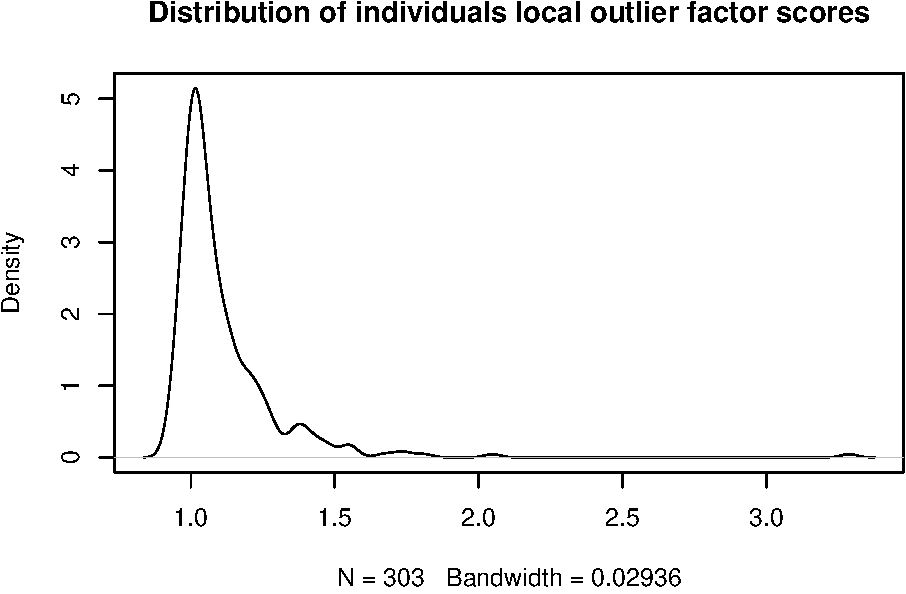
\includegraphics{project_report_files/figure-latex/unnamed-chunk-4-1.pdf}

\begin{Shaded}
\begin{Highlighting}[]
\CommentTok{#Exploratory Data Analysis}
\CommentTok{#Density of heart presence/absence disease by age}
\NormalTok{g1 <-}\StringTok{ }\KeywordTok{ggplot}\NormalTok{(}\DataTypeTok{data=}\NormalTok{heart_disease, }\KeywordTok{aes}\NormalTok{(}\DataTypeTok{x=}\NormalTok{X...age, }\DataTypeTok{fill=}\KeywordTok{as.factor}\NormalTok{(target)))}\OperatorTok{+}
\StringTok{  }\KeywordTok{geom_density}\NormalTok{(}\DataTypeTok{alpha=}\NormalTok{.}\DecValTok{5}\NormalTok{)}\OperatorTok{+}
\StringTok{  }\KeywordTok{ggtitle}\NormalTok{(}\StringTok{"Age"}\NormalTok{) }\OperatorTok{+}
\StringTok{  }\KeywordTok{scale_fill_manual}\NormalTok{(}\DataTypeTok{values =} \KeywordTok{c}\NormalTok{(}\StringTok{'skyblue4'}\NormalTok{, }\StringTok{'skyblue2'}\NormalTok{),}\DataTypeTok{name =} \StringTok{"Disease"}\NormalTok{, }\DataTypeTok{labels =} \KeywordTok{c}\NormalTok{(}\StringTok{"Yes"}\NormalTok{, }\StringTok{"No"}\NormalTok{))}

\CommentTok{#Density of heart presence/absence disease by Max heart rate}
\NormalTok{g2 <-}\StringTok{ }\KeywordTok{ggplot}\NormalTok{(}\DataTypeTok{data=}\NormalTok{heart_disease, }\KeywordTok{aes}\NormalTok{(}\DataTypeTok{x=}\NormalTok{thalach, }\DataTypeTok{fill=}\KeywordTok{as.factor}\NormalTok{(target)))}\OperatorTok{+}
\StringTok{  }\KeywordTok{geom_density}\NormalTok{(}\DataTypeTok{alpha=}\NormalTok{.}\DecValTok{5}\NormalTok{)}\OperatorTok{+}
\StringTok{  }\KeywordTok{ggtitle}\NormalTok{(}\StringTok{"Max Hear Rate"}\NormalTok{) }\OperatorTok{+}
\StringTok{  }\KeywordTok{scale_fill_manual}\NormalTok{(}\DataTypeTok{values =} \KeywordTok{c}\NormalTok{(}\StringTok{'skyblue4'}\NormalTok{, }\StringTok{'skyblue2'}\NormalTok{),}\DataTypeTok{name =} \StringTok{"Disease"}\NormalTok{, }\DataTypeTok{labels =} \KeywordTok{c}\NormalTok{(}\StringTok{"Yes"}\NormalTok{, }\StringTok{"No"}\NormalTok{))}

\CommentTok{#Density of heart presence/absence disease by sex}
\NormalTok{g3 <-}\StringTok{ }\KeywordTok{ggplot}\NormalTok{(}\DataTypeTok{data=}\NormalTok{heart_disease, }\KeywordTok{aes}\NormalTok{(}\DataTypeTok{x=}\NormalTok{sex, }\DataTypeTok{fill=}\KeywordTok{as.factor}\NormalTok{(target)))}\OperatorTok{+}
\StringTok{      }\KeywordTok{geom_bar}\NormalTok{(}\DataTypeTok{alpha=}\NormalTok{.}\DecValTok{5}\NormalTok{, }\DataTypeTok{color=}\StringTok{"black"}\NormalTok{)}\OperatorTok{+}
\StringTok{      }\KeywordTok{ggtitle}\NormalTok{(}\StringTok{"Sex"}\NormalTok{) }\OperatorTok{+}
\StringTok{      }\KeywordTok{scale_fill_manual}\NormalTok{(}\DataTypeTok{values =} \KeywordTok{c}\NormalTok{(}\StringTok{'skyblue4'}\NormalTok{, }\StringTok{'skyblue2'}\NormalTok{),}\DataTypeTok{name =} \StringTok{"Disease"}\NormalTok{, }\DataTypeTok{labels =} \KeywordTok{c}\NormalTok{(}\StringTok{"Yes"}\NormalTok{, }\StringTok{"No"}\NormalTok{))}

\CommentTok{#Density of heart presence/absence disease by chest type}
\NormalTok{g4 <-}\StringTok{ }\KeywordTok{ggplot}\NormalTok{(}\DataTypeTok{data=}\NormalTok{heart_disease, }\KeywordTok{aes}\NormalTok{(}\DataTypeTok{x=}\NormalTok{cp, }\DataTypeTok{fill=}\KeywordTok{as.factor}\NormalTok{(target)))}\OperatorTok{+}
\StringTok{  }\KeywordTok{geom_bar}\NormalTok{(}\DataTypeTok{alpha=}\NormalTok{.}\DecValTok{5}\NormalTok{, }\DataTypeTok{color=}\StringTok{"black"}\NormalTok{)}\OperatorTok{+}
\StringTok{  }\KeywordTok{ggtitle}\NormalTok{(}\StringTok{"Chest Pain type"}\NormalTok{) }\OperatorTok{+}
\StringTok{  }\KeywordTok{scale_fill_manual}\NormalTok{(}\DataTypeTok{values =} \KeywordTok{c}\NormalTok{(}\StringTok{'skyblue4'}\NormalTok{, }\StringTok{'skyblue2'}\NormalTok{),}\DataTypeTok{name =} \StringTok{"Disease"}\NormalTok{, }\DataTypeTok{labels =} \KeywordTok{c}\NormalTok{(}\StringTok{"Yes"}\NormalTok{, }\StringTok{"No"}\NormalTok{))}

\KeywordTok{grid.arrange}\NormalTok{(g1, g2, g3, g4, }\DataTypeTok{ncol =} \DecValTok{2}\NormalTok{)}
\end{Highlighting}
\end{Shaded}

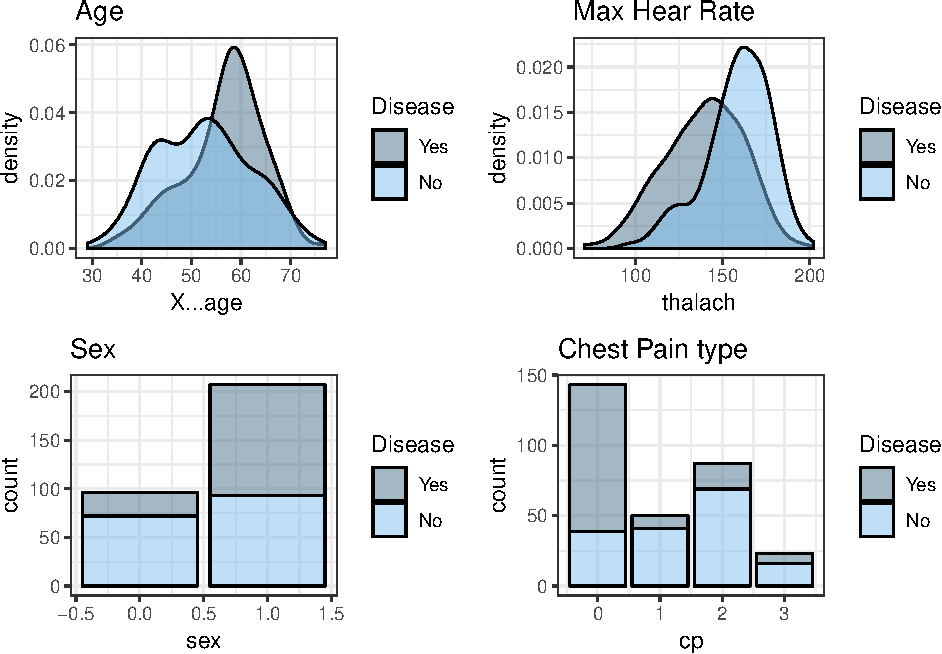
\includegraphics{project_report_files/figure-latex/unnamed-chunk-5-1.pdf}

\begin{Shaded}
\begin{Highlighting}[]
\KeywordTok{plot_correlation}\NormalTok{(heart_disease)}
\end{Highlighting}
\end{Shaded}

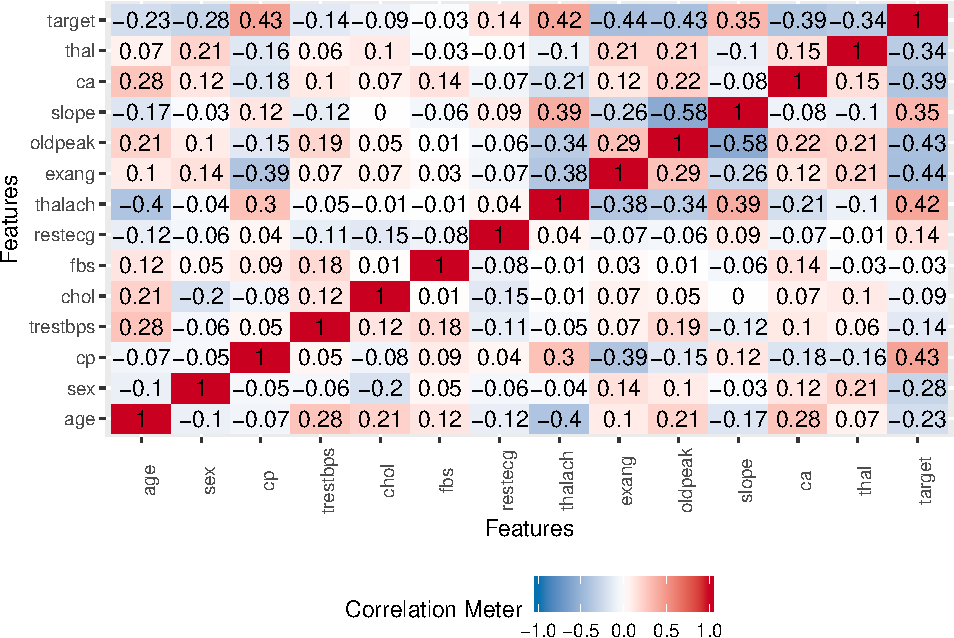
\includegraphics{project_report_files/figure-latex/unnamed-chunk-6-1.pdf}

\begin{Shaded}
\begin{Highlighting}[]
\CommentTok{#PCA with categoriacal values}
\NormalTok{pca_facto <-}\StringTok{ }\NormalTok{factor_heart[, }\KeywordTok{sapply}\NormalTok{(factor_heart, class) }\OperatorTok{!=}\StringTok{ "factor"}\NormalTok{]}
\CommentTok{#Some categorical values can be added as supplementary}
\CommentTok{#pca_facto$sex <- factor_heart$sex}
\CommentTok{#pca_facto$ca <- factor_heart$ca}
\NormalTok{pca_facto}\OperatorTok{$}\NormalTok{disease <-}\StringTok{ }\NormalTok{heart_disease}\OperatorTok{$}\NormalTok{target}
\NormalTok{pca_facto}\OperatorTok{$}\NormalTok{disease[pca_facto}\OperatorTok{$}\NormalTok{disease}\OperatorTok{==}\DecValTok{0}\NormalTok{] <-}\StringTok{ "Yes"}
\NormalTok{pca_facto}\OperatorTok{$}\NormalTok{disease[pca_facto}\OperatorTok{$}\NormalTok{disease}\OperatorTok{==}\DecValTok{1}\NormalTok{] <-}\StringTok{ "No"}

\NormalTok{pca_facto_heart <-}\StringTok{ }\KeywordTok{PCA}\NormalTok{(pca_facto, }\DataTypeTok{quali.sup =} \DecValTok{6}\NormalTok{, }\DataTypeTok{scale.unit =} \OtherTok{TRUE}\NormalTok{,  }\DataTypeTok{graph =} \OtherTok{TRUE}\NormalTok{)}
\end{Highlighting}
\end{Shaded}

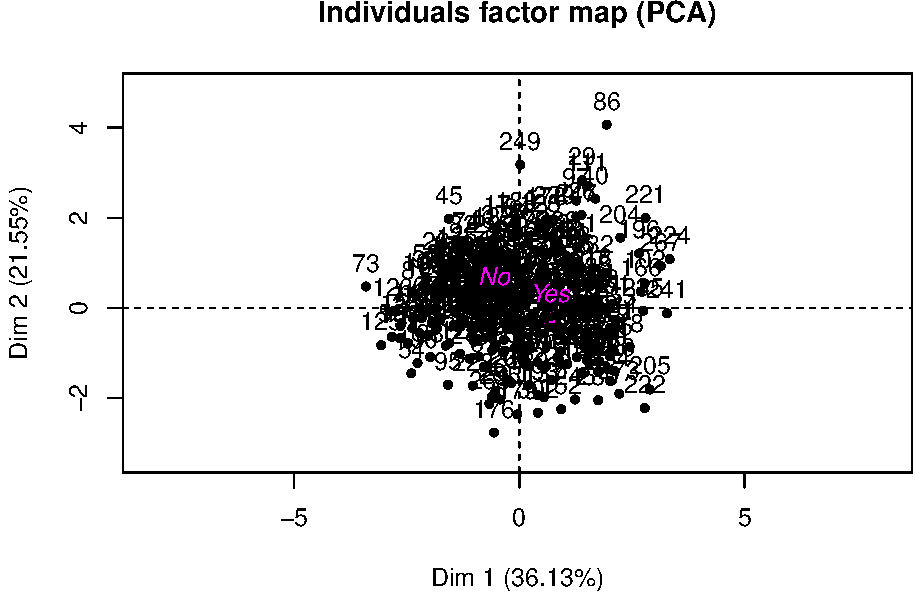
\includegraphics{project_report_files/figure-latex/unnamed-chunk-7-1.pdf}
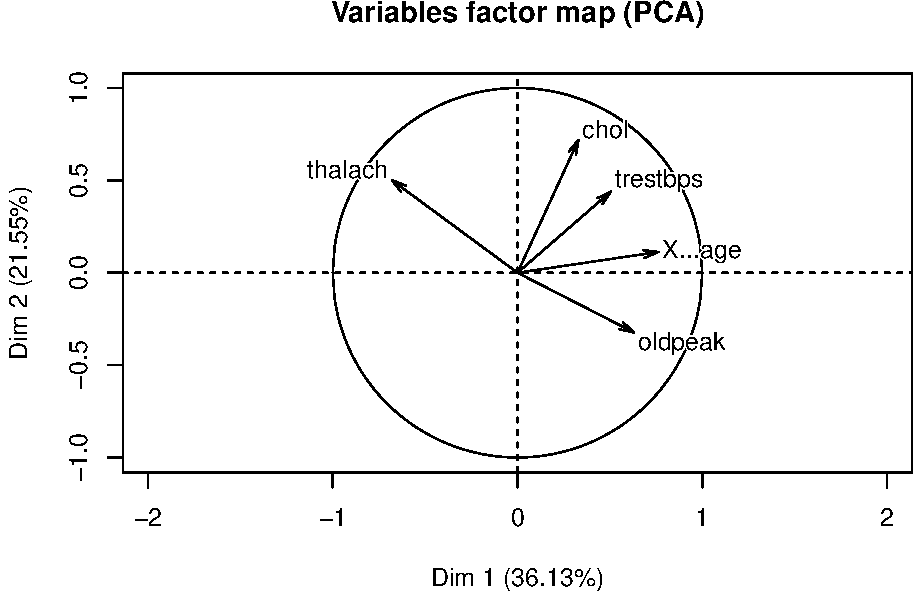
\includegraphics{project_report_files/figure-latex/unnamed-chunk-7-2.pdf}

\begin{Shaded}
\begin{Highlighting}[]
\CommentTok{#Screeplots}
\KeywordTok{fviz_screeplot}\NormalTok{(pca_facto_heart, }\DataTypeTok{addlabels =} \OtherTok{FALSE}\NormalTok{)}
\end{Highlighting}
\end{Shaded}

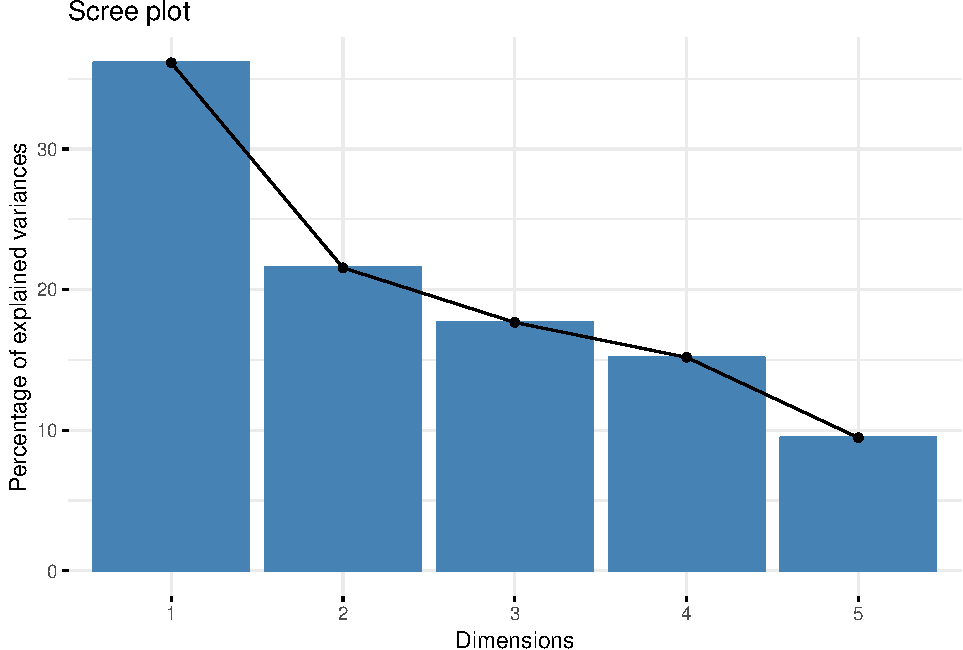
\includegraphics{project_report_files/figure-latex/unnamed-chunk-8-1.pdf}

\begin{Shaded}
\begin{Highlighting}[]
\NormalTok{eigen_values <-}\StringTok{ }\NormalTok{pca_facto_heart}\OperatorTok{$}\NormalTok{eig[,}\DecValTok{1}\NormalTok{]}
\KeywordTok{plot}\NormalTok{(eigen_values, }\DataTypeTok{type=}\StringTok{"o"}\NormalTok{, }\DataTypeTok{main=}\StringTok{"Screeplot"}\NormalTok{, }
     \DataTypeTok{xlab=}\StringTok{'Dimension'}\NormalTok{, }\DataTypeTok{ylab=}\StringTok{'Eigenvalue'}\NormalTok{, }\DataTypeTok{col=}\StringTok{'blue'}\NormalTok{)}
\KeywordTok{abline}\NormalTok{(}\DataTypeTok{h=}\DecValTok{1}\NormalTok{,}\DataTypeTok{col=}\StringTok{"red"}\NormalTok{)}
\end{Highlighting}
\end{Shaded}

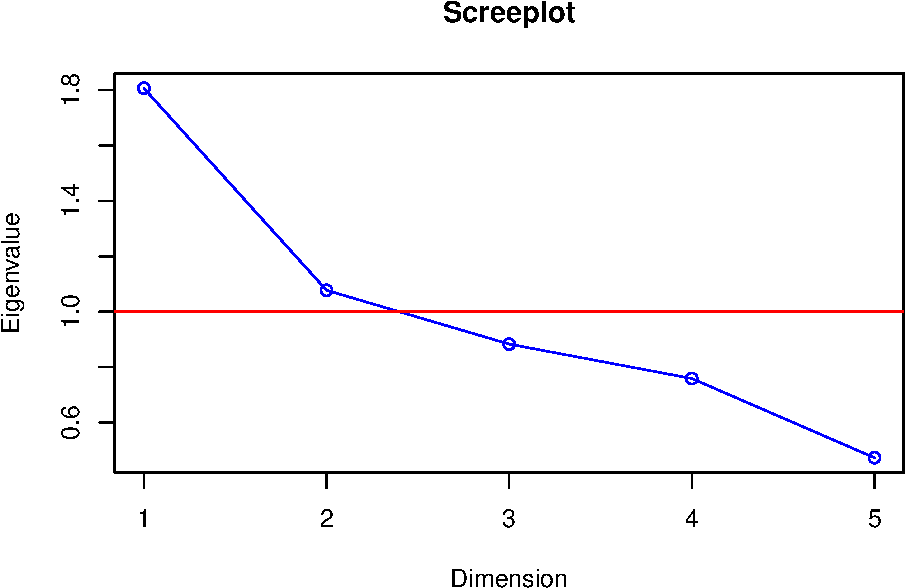
\includegraphics{project_report_files/figure-latex/unnamed-chunk-8-2.pdf}

\begin{Shaded}
\begin{Highlighting}[]
\CommentTok{#Represented in Rp}
\CommentTok{#quali.sup -> Every modality is the centroide of the respective individuals having chosen that modality}
\KeywordTok{fviz_pca_ind}\NormalTok{(pca_facto_heart, }\DataTypeTok{habillage =} \DecValTok{6}\NormalTok{, }\DataTypeTok{geom =} \StringTok{"point"}\NormalTok{, }\DataTypeTok{label=}\StringTok{"quali"}\NormalTok{,}\DataTypeTok{addEllipses =}\OtherTok{TRUE}\NormalTok{, }\DataTypeTok{ellipse.level =} \FloatTok{0.68}\NormalTok{)}\CommentTok{#co l.ind='cos2'}
\end{Highlighting}
\end{Shaded}

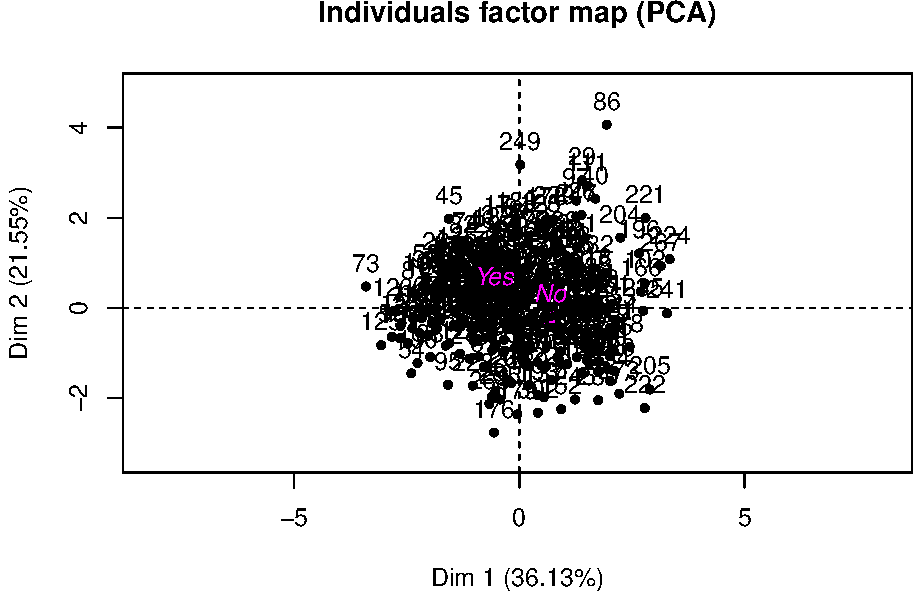
\includegraphics{project_report_files/figure-latex/unnamed-chunk-9-1.pdf}

\begin{Shaded}
\begin{Highlighting}[]
\KeywordTok{plot.PCA}\NormalTok{(pca_facto_heart, }\DataTypeTok{quali.sup =} \DecValTok{6}\NormalTok{, }\DataTypeTok{scale.unit =} \OtherTok{TRUE}\NormalTok{,}\DataTypeTok{choix =} \StringTok{'ind'}\NormalTok{,}\DataTypeTok{label=}\StringTok{"quali"}\NormalTok{)}
\end{Highlighting}
\end{Shaded}

\begin{verbatim}
## Warning in plot.window(...): "quali.sup" is not a graphical parameter
\end{verbatim}

\begin{verbatim}
## Warning in plot.window(...): "scale.unit" is not a graphical parameter
\end{verbatim}

\begin{verbatim}
## Warning in plot.xy(xy, type, ...): "quali.sup" is not a graphical parameter
\end{verbatim}

\begin{verbatim}
## Warning in plot.xy(xy, type, ...): "scale.unit" is not a graphical
## parameter
\end{verbatim}

\begin{verbatim}
## Warning in axis(side = side, at = at, labels = labels, ...): "quali.sup" is
## not a graphical parameter
\end{verbatim}

\begin{verbatim}
## Warning in axis(side = side, at = at, labels = labels, ...): "scale.unit"
## is not a graphical parameter
\end{verbatim}

\begin{verbatim}
## Warning in axis(side = side, at = at, labels = labels, ...): "quali.sup" is
## not a graphical parameter
\end{verbatim}

\begin{verbatim}
## Warning in axis(side = side, at = at, labels = labels, ...): "scale.unit"
## is not a graphical parameter
\end{verbatim}

\begin{verbatim}
## Warning in box(...): "quali.sup" is not a graphical parameter
\end{verbatim}

\begin{verbatim}
## Warning in box(...): "scale.unit" is not a graphical parameter
\end{verbatim}

\begin{verbatim}
## Warning in title(...): "quali.sup" is not a graphical parameter
\end{verbatim}

\begin{verbatim}
## Warning in title(...): "scale.unit" is not a graphical parameter
\end{verbatim}

\begin{verbatim}
## Warning in int_abline(a = a, b = b, h = h, v = v, untf = untf, ...):
## "quali.sup" is not a graphical parameter
\end{verbatim}

\begin{verbatim}
## Warning in int_abline(a = a, b = b, h = h, v = v, untf = untf, ...):
## "scale.unit" is not a graphical parameter
\end{verbatim}

\begin{verbatim}
## Warning in int_abline(a = a, b = b, h = h, v = v, untf = untf, ...):
## "quali.sup" is not a graphical parameter
\end{verbatim}

\begin{verbatim}
## Warning in int_abline(a = a, b = b, h = h, v = v, untf = untf, ...):
## "scale.unit" is not a graphical parameter
\end{verbatim}

\begin{verbatim}
## Warning in plot.xy(xy.coords(x, y), type = type, ...): "quali.sup" is not a
## graphical parameter
\end{verbatim}

\begin{verbatim}
## Warning in plot.xy(xy.coords(x, y), type = type, ...): "scale.unit" is not
## a graphical parameter
\end{verbatim}

\begin{verbatim}
## Warning in text.default(xy, labels, cex = cex, ...): "quali.sup" is not a
## graphical parameter
\end{verbatim}

\begin{verbatim}
## Warning in text.default(xy, labels, cex = cex, ...): "scale.unit" is not a
## graphical parameter
\end{verbatim}

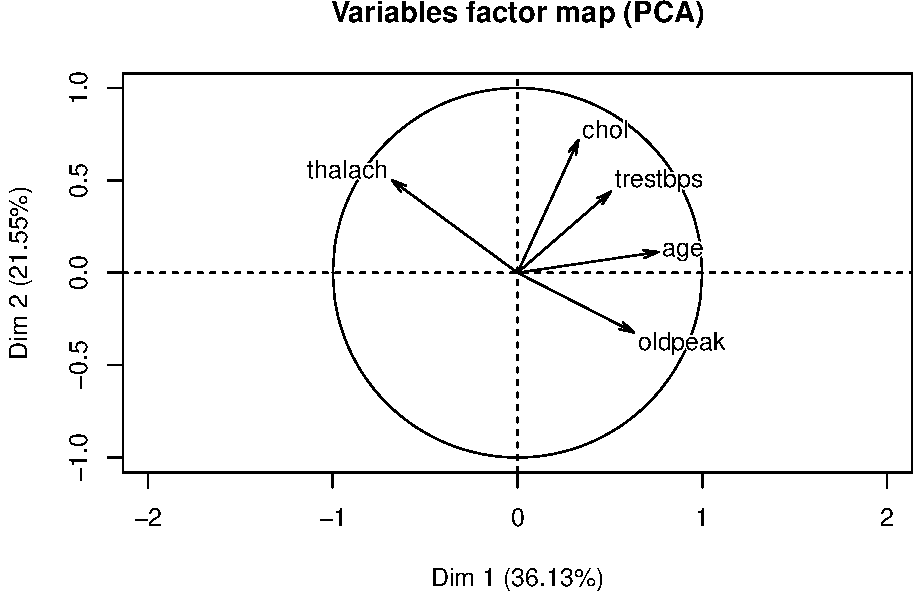
\includegraphics{project_report_files/figure-latex/unnamed-chunk-9-2.pdf}

\begin{Shaded}
\begin{Highlighting}[]
\CommentTok{#Represented in Rn}
\CommentTok{#Projection of variables, show correlation between principal components}
\KeywordTok{fviz_pca_var}\NormalTok{(pca_facto_heart, }\DataTypeTok{geom =} \KeywordTok{c}\NormalTok{(}\StringTok{"arrow"}\NormalTok{, }\StringTok{"text"}\NormalTok{), }\DataTypeTok{col.var =} \StringTok{"cos2"}\NormalTok{)}\CommentTok{#By quality of representation cos2}
\end{Highlighting}
\end{Shaded}

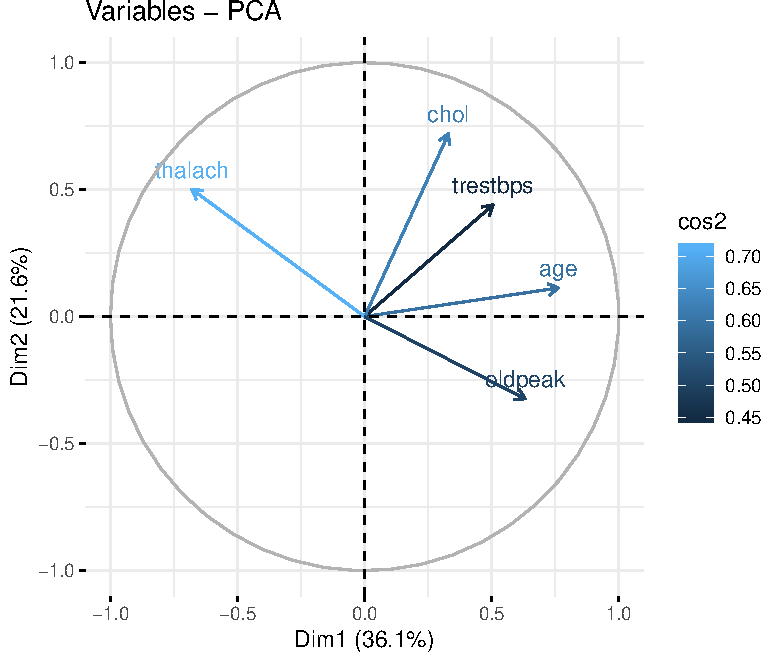
\includegraphics{project_report_files/figure-latex/unnamed-chunk-10-1.pdf}

\begin{Shaded}
\begin{Highlighting}[]
\NormalTok{proj_indiv <-}\StringTok{ }\NormalTok{pca_facto_heart}\OperatorTok{$}\NormalTok{ind}\OperatorTok{$}\NormalTok{coord[,}\DecValTok{1}\OperatorTok{:}\DecValTok{2}\NormalTok{] }\CommentTok{#individual projections on 1st factorial plane}
\CommentTok{#Clustering}
\NormalTok{hc_ward =}\StringTok{ }\KeywordTok{hclust}\NormalTok{(}\KeywordTok{dist}\NormalTok{(proj_indiv),}\DataTypeTok{method =} \StringTok{"ward.D"}\NormalTok{)}
\KeywordTok{plot}\NormalTok{(hc_ward, }\DataTypeTok{main=} \StringTok{"HC using Ward Agglomeration method"}\NormalTok{, }\DataTypeTok{xlab=}\StringTok{""}\NormalTok{,}\DataTypeTok{sub=}\StringTok{""}\NormalTok{,}\DataTypeTok{cex=}\NormalTok{.}\DecValTok{9}\NormalTok{,  }\DataTypeTok{labels=}\OtherTok{FALSE}\NormalTok{)}
\KeywordTok{abline}\NormalTok{(}\DataTypeTok{h=}\DecValTok{60}\NormalTok{)}
\KeywordTok{rect.hclust}\NormalTok{(hc_ward, }\DataTypeTok{k =} \DecValTok{3}\NormalTok{, }\DataTypeTok{border =} \DecValTok{2}\OperatorTok{:}\DecValTok{6}\NormalTok{)}
\end{Highlighting}
\end{Shaded}

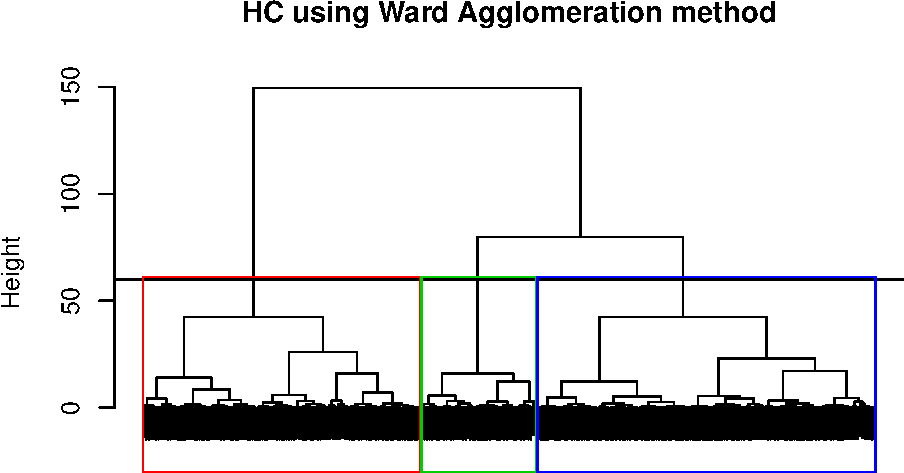
\includegraphics{project_report_files/figure-latex/unnamed-chunk-11-1.pdf}

\begin{Shaded}
\begin{Highlighting}[]
\CommentTok{#Association of individuals to clusters}
\NormalTok{classes <-}\StringTok{ }\KeywordTok{cutree}\NormalTok{(hc_ward, }\DataTypeTok{h=}\DecValTok{50}\NormalTok{) }\CommentTok{#Depending on the height, number of clusters is chosen}
\KeywordTok{plotcluster}\NormalTok{(proj_indiv, classes,}\DataTypeTok{main=}\StringTok{"Projections of individuals in Hierarchical Clustering of 3 classes"}\NormalTok{)}
\end{Highlighting}
\end{Shaded}

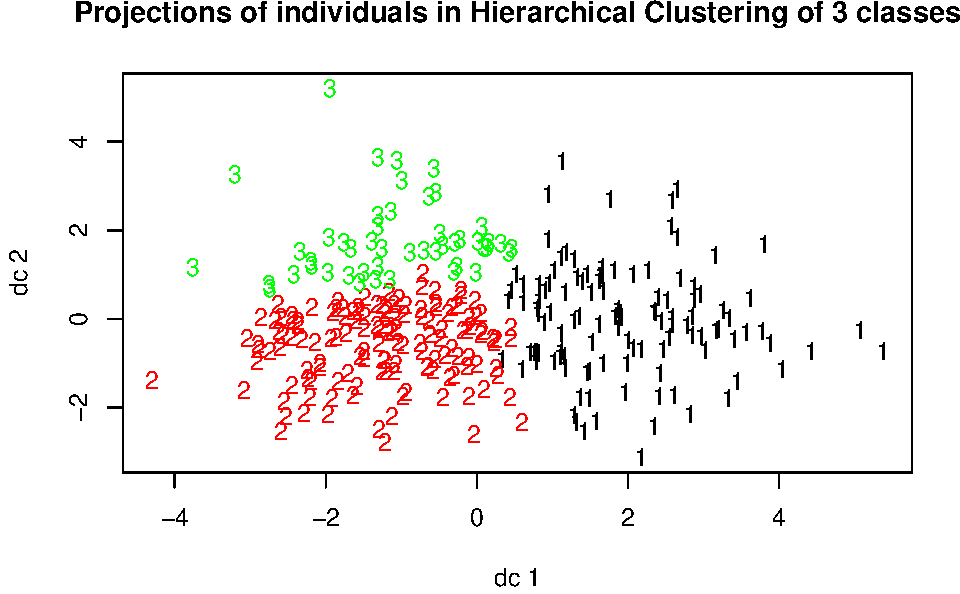
\includegraphics{project_report_files/figure-latex/unnamed-chunk-11-2.pdf}

\begin{Shaded}
\begin{Highlighting}[]
\NormalTok{get_centroids <-}\StringTok{ }\ControlFlowTok{function}\NormalTok{(classes, n_classes)\{}
\NormalTok{  centroids <-}\StringTok{ }\OtherTok{NULL}
  \ControlFlowTok{for}\NormalTok{(k }\ControlFlowTok{in} \DecValTok{1}\OperatorTok{:}\NormalTok{n_classes)\{}
\NormalTok{    centroids <-}\StringTok{ }\KeywordTok{rbind}\NormalTok{(centroids, }\KeywordTok{colMeans}\NormalTok{(proj_indiv[classes }\OperatorTok{==}\StringTok{ }\NormalTok{k, , }\DataTypeTok{drop =} \OtherTok{FALSE}\NormalTok{]))}
\NormalTok{  \}}
  \KeywordTok{return}\NormalTok{(centroids)}
\NormalTok{\}}
\NormalTok{centroids <-}\StringTok{ }\KeywordTok{get_centroids}\NormalTok{(classes, }\DecValTok{3}\NormalTok{)}
\end{Highlighting}
\end{Shaded}

\begin{Shaded}
\begin{Highlighting}[]
\CommentTok{#k_mean needs centroid of clusters}
\NormalTok{k_mean <-}\StringTok{ }\KeywordTok{kmeans}\NormalTok{(proj_indiv, centroids)}
\KeywordTok{plotcluster}\NormalTok{(proj_indiv, k_mean}\OperatorTok{$}\NormalTok{cluster,}\DataTypeTok{main=}\StringTok{"Projections of individuals in K-means Clustering of 3 classes"}\NormalTok{)}
\end{Highlighting}
\end{Shaded}

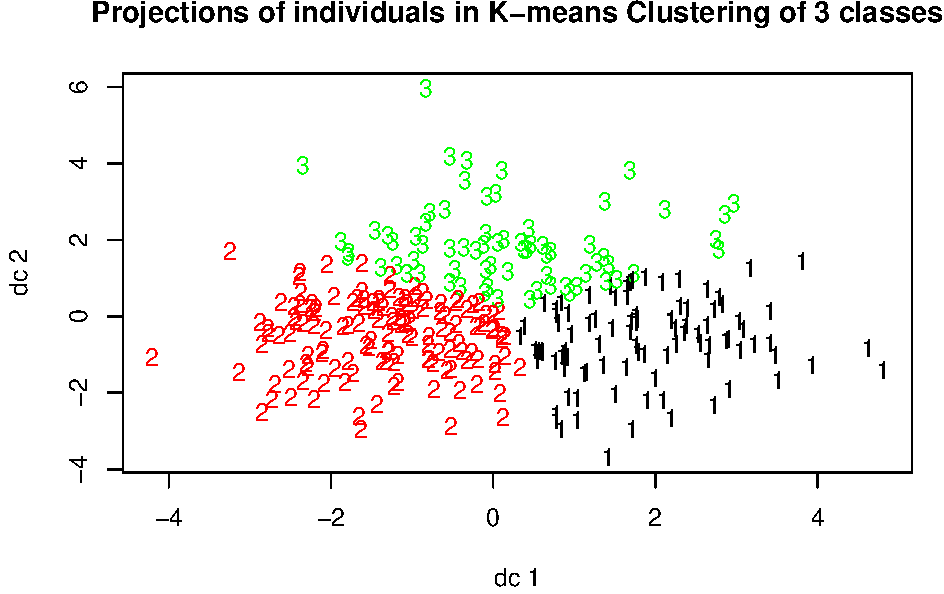
\includegraphics{project_report_files/figure-latex/unnamed-chunk-13-1.pdf}

\begin{Shaded}
\begin{Highlighting}[]
\NormalTok{cal_idx_before <-}\StringTok{ }\KeywordTok{calinhara}\NormalTok{(proj_indiv,classes,}\DataTypeTok{cn=}\KeywordTok{max}\NormalTok{(classes))}
\NormalTok{cal_idx_after <-}\StringTok{ }\KeywordTok{calinhara}\NormalTok{(proj_indiv,k_mean}\OperatorTok{$}\NormalTok{cluster,}\DataTypeTok{cn=}\KeywordTok{max}\NormalTok{(k_mean}\OperatorTok{$}\NormalTok{cluster))}

\KeywordTok{print}\NormalTok{(cal_idx_before)}
\end{Highlighting}
\end{Shaded}

\begin{verbatim}
## [1] 198.1154
\end{verbatim}

\begin{Shaded}
\begin{Highlighting}[]
\KeywordTok{print}\NormalTok{(cal_idx_after)}
\end{Highlighting}
\end{Shaded}

\begin{verbatim}
## [1] 226.1952
\end{verbatim}

\begin{Shaded}
\begin{Highlighting}[]
\CommentTok{#Improvement}
\end{Highlighting}
\end{Shaded}

\begin{Shaded}
\begin{Highlighting}[]
\NormalTok{Calinski_Harabassza <-}\StringTok{ }\ControlFlowTok{function}\NormalTok{ (projections, hc, kind, n_classes)\{}
\NormalTok{  classes <-}\StringTok{ }\KeywordTok{cutree}\NormalTok{(hc, }\DataTypeTok{k=}\NormalTok{n_classes)}
\NormalTok{  centroids <-}\StringTok{ }\KeywordTok{get_centroids}\NormalTok{(classes, n_classes)}
  \ControlFlowTok{if}\NormalTok{(kind}\OperatorTok{==}\StringTok{'hc'}\NormalTok{)\{}
\NormalTok{    index <-}\StringTok{ }\KeywordTok{calinhara}\NormalTok{(proj_indiv,classes,}\DataTypeTok{cn=}\KeywordTok{max}\NormalTok{(classes))}
\NormalTok{  \}}
  \ControlFlowTok{if}\NormalTok{(kind}\OperatorTok{==}\StringTok{'kmeans'}\NormalTok{)\{}
\NormalTok{    kmeans_classes <-}\StringTok{ }\KeywordTok{kmeans}\NormalTok{(proj_indiv, }\DataTypeTok{centers =}\NormalTok{ centroids)}\OperatorTok{$}\NormalTok{cluster}
\NormalTok{    index <-}\KeywordTok{calinhara}\NormalTok{(proj_indiv,kmeans_classes,}\DataTypeTok{cn=}\KeywordTok{max}\NormalTok{(kmeans_classes)) }
\NormalTok{  \}}
  \KeywordTok{return}\NormalTok{(index)}
\NormalTok{\}}
\NormalTok{get_indexes <-}\StringTok{ }\ControlFlowTok{function}\NormalTok{(until, kind)\{}
\NormalTok{  indexes <-}\StringTok{ }\KeywordTok{c}\NormalTok{()}
  \ControlFlowTok{for}\NormalTok{ (n_classes }\ControlFlowTok{in} \DecValTok{2}\OperatorTok{:}\NormalTok{until)\{}
\NormalTok{    indexes <-}\StringTok{ }\KeywordTok{c}\NormalTok{(indexes, }\KeywordTok{Calinski_Harabassza}\NormalTok{(proj_indiv, hc_ward, kind, n_classes))}
\NormalTok{  \}  }
  \KeywordTok{return}\NormalTok{(indexes)}
\NormalTok{\}}
\end{Highlighting}
\end{Shaded}

\begin{Shaded}
\begin{Highlighting}[]
\NormalTok{indexes_before <-}\StringTok{ }\KeywordTok{get_indexes}\NormalTok{(}\DecValTok{10}\NormalTok{, }\StringTok{'hc'}\NormalTok{)}
\KeywordTok{plot}\NormalTok{(indexes_before, }\DataTypeTok{type =} \StringTok{"o"}\NormalTok{, }\DataTypeTok{xlab =} \StringTok{'Number of classes'}\NormalTok{, }\DataTypeTok{ylab =} \StringTok{'Calinski index value'}
\NormalTok{, }\DataTypeTok{main =} \StringTok{'Index before consolidation'}\NormalTok{, }\DataTypeTok{col =} \StringTok{'blue'}\NormalTok{, xaxt}
\NormalTok{=}\StringTok{ "n"}\NormalTok{)}
\KeywordTok{axis}\NormalTok{(}\DecValTok{1}\NormalTok{, }\DataTypeTok{at=}\DecValTok{1}\OperatorTok{:}\DecValTok{9}\NormalTok{, }\DataTypeTok{labels =} \KeywordTok{c}\NormalTok{(}\DecValTok{2}\NormalTok{, }\DecValTok{3}\NormalTok{, }\DecValTok{4}\NormalTok{, }\DecValTok{5}\NormalTok{, }\DecValTok{6}\NormalTok{, }\DecValTok{7}\NormalTok{,}\DecValTok{8}\NormalTok{,}\DecValTok{9}\NormalTok{,}\DecValTok{10}\NormalTok{))  }
\end{Highlighting}
\end{Shaded}

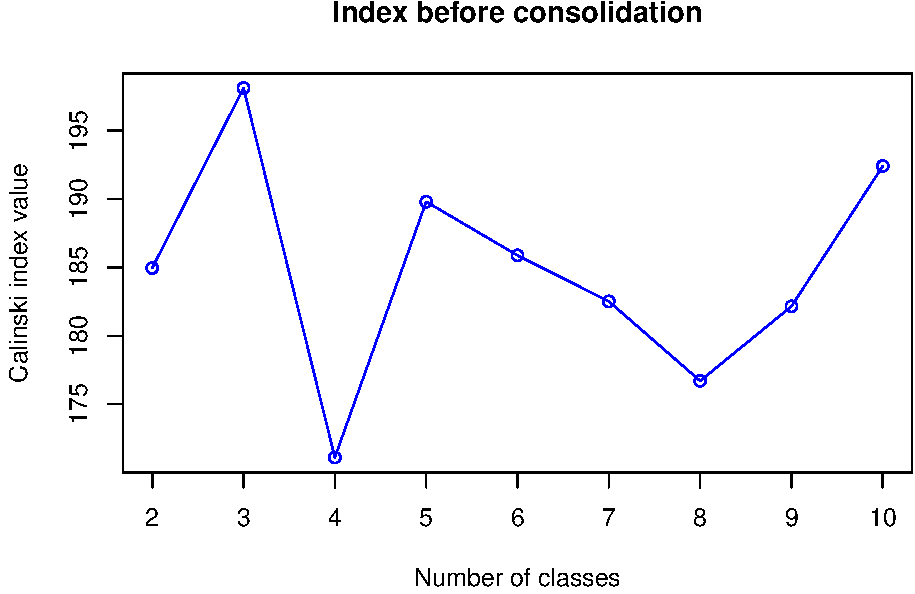
\includegraphics{project_report_files/figure-latex/unnamed-chunk-16-1.pdf}

\begin{Shaded}
\begin{Highlighting}[]
\NormalTok{indexes_after <-}\StringTok{ }\KeywordTok{get_indexes}\NormalTok{(}\DecValTok{10}\NormalTok{, }\StringTok{'kmeans'}\NormalTok{)}
\KeywordTok{plot}\NormalTok{(indexes_after, }\DataTypeTok{type =} \StringTok{"o"}\NormalTok{, }\DataTypeTok{xlab =} \StringTok{'Number of classes'}\NormalTok{, }\DataTypeTok{ylab =} \StringTok{'Calinski index value'}
\NormalTok{, }\DataTypeTok{main =} \StringTok{'Index after consolidation'}\NormalTok{, }\DataTypeTok{col =} \StringTok{'blue'}\NormalTok{, xaxt}
\NormalTok{=}\StringTok{ "n"}\NormalTok{)}
\KeywordTok{axis}\NormalTok{(}\DecValTok{1}\NormalTok{, }\DataTypeTok{at=}\DecValTok{1}\OperatorTok{:}\DecValTok{9}\NormalTok{, }\DataTypeTok{labels =} \KeywordTok{c}\NormalTok{(}\DecValTok{2}\NormalTok{, }\DecValTok{3}\NormalTok{, }\DecValTok{4}\NormalTok{, }\DecValTok{5}\NormalTok{, }\DecValTok{6}\NormalTok{, }\DecValTok{7}\NormalTok{,}\DecValTok{8}\NormalTok{,}\DecValTok{9}\NormalTok{,}\DecValTok{10}\NormalTok{))  }
\end{Highlighting}
\end{Shaded}

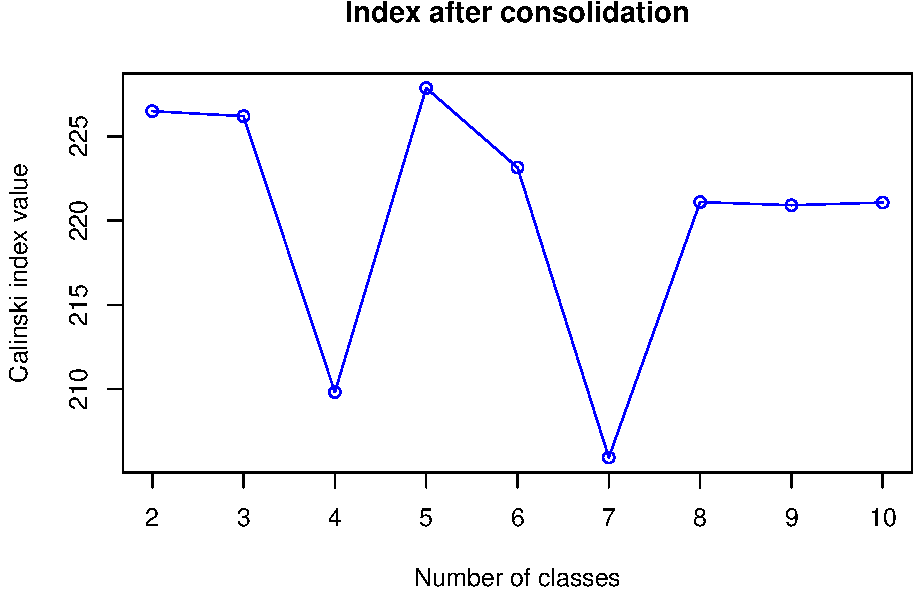
\includegraphics{project_report_files/figure-latex/unnamed-chunk-17-1.pdf}


\end{document}
